
\blank
\newpage

\section{Retrieval-Augmented Generation}

    \begin{wrapfigure}{r}{0.5\textwidth}
        \vspace{-15pt}
        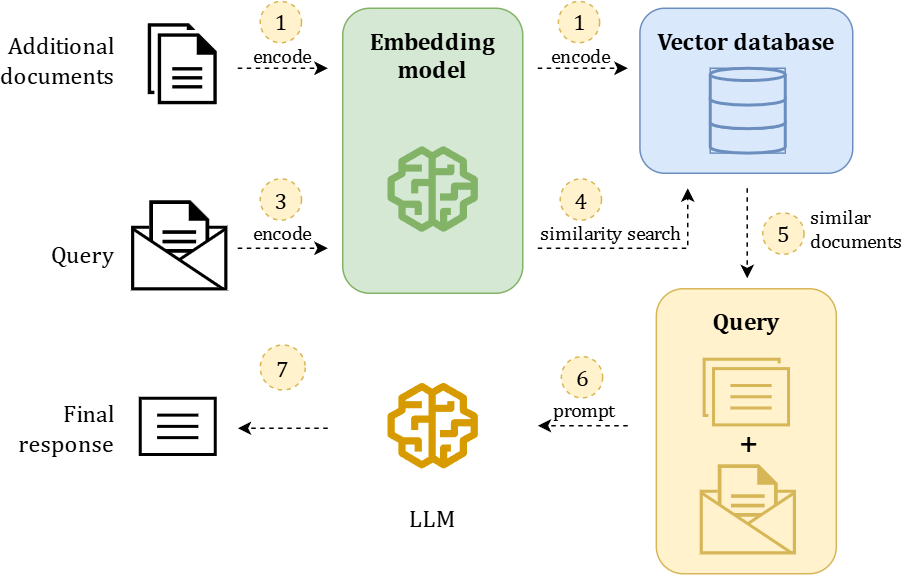
\includegraphics[width=1\linewidth]{imgs/schema_12_1.png}
        \label{fig:fig121}
    \end{wrapfigure}

    La \textit{Retrieval-Augmented Generation} (RAG) è una tecnica avanzata che combina il recupero di informazioni (\textit{retrieval}) e la generazione di testo (\textit{generation}) per migliorare le capacità di un Large Language Model (LLM) senza la necessità di effettuare il \textit{fine-tuning} del modello stesso. 

    Rispetto a un Base LLM (soggetto ad allucinazioni e privo di informazioni aggiornate) o a un FT LLM (che richiede costi elevati di addestramento), un sistema RAG offre risposte di alta qualità, accesso a informazioni aggiornate e un maggior controllo sui dati generati, il tutto con costi contenuti (\textit{on-budget}).

    Dal punto di vista concettuale, l'architettura RAG si basa su due tipi di memoria:
    
    \begin{itemize}
        \item \textbf{Memoria non-parametrica}: Gestita dal \textit{retriever}, che è statico e non possiede pesi apprendibili.
        \item \textbf{Memoria parametrica}: Gestita dal \textit{generator} (il LLM), la cui conoscenza dipende dai pesi appresi in fase di addestramento.
    \end{itemize}

    \subsection{Componenti dell'Architettura RAG}

        \subsubsection{Corpus ed Embeddings}
        
            I dati di dominio (come documenti testuali, JSON o dati privati) costituiscono la \textit{Knowledge Base}. Questi documenti vengono suddivisi in piccole sezioni chiamate \textit{chunk}. Successivamente, un modello linguistico dedicato (\textit{Embedding LLM}) codifica i chunk trasformandoli in rappresentazioni vettoriali dense (\textit{embedding}).

        \subsubsection{Retriever e Vector Store}
        
            L'obiettivo del \textit{retriever} è estrarre i documenti più rilevanti per una data \textit{query} utente, al fine di arricchire il contesto del generatore. I chunk vettorializzati vengono memorizzati in un \textit{vector store} (come Chroma, Faiss, Pinecone o Neo4j), un database indicizzato che permette memorizzazione e accesso efficienti.

            Il recupero avviene tramite una \textit{similarity function} che ordina i migliori $k$ chunk estratti. Oltre alla classica \textit{cosine similarity}, si utilizza spesso il criterio della \textit{Maximum Marginal Relevance (MMR)} per bilanciare la rilevanza rispetto alla query e la diversità dei documenti estratti. La formula del MMR è:
            $$MMR = \arg\max_{D_i \in R \setminus S} \left[ \lambda \cdot Sim_1(D_i, Q) - (1 - \lambda) \cdot \max_{D_j \in S} Sim_2(D_i, D_j) \right]$$
            dove:
            
            \begin{itemize}
                \item $Q$ è la query dell'utente.
                \item $R$ è la lista dei chunk candidati recuperati dal retriever.
                \item $S$ è l'insieme dei documenti già selezionati per il contesto.
                \item $\lambda \in [0, 1]$ regola il compromesso: $\lambda = 1$ massimizza la rilevanza rispetto alla query, mentre $\lambda = 0$ favorisce la massima diversità.
            \end{itemize}

        \subsubsection{Generator}
        
            Il generatore è tipicamente un LLM \textit{decoder-only}. Riceve in input un \textit{prompt} strutturato contenente l'istruzione di base, il contesto (i documenti recuperati) e la domanda dell'utente. Basandosi esclusivamente su tali informazioni, il modello genera la risposta finale.

    \newpage

    \subsection{Valutazione dei Sistemi RAG}
    
        La valutazione di un sistema RAG si divide tra le prestazioni del recupero e quelle della generazione:
        
        \begin{itemize}
            \item \textbf{Retriever}: Si valuta la \textit{Precision}, l'\textit{Accuracy} e la pertinenza del contesto (\textit{Context relevancy}), spesso tramite tecniche di \textit{LLM as a judge} o valutazione umana.
            \item \textbf{Generator}: Si valuta la qualità testuale con metriche tradizionali (BLEU, ROUGE, BERT-score, Perplexity) e l'affidabilità (\textit{Faithfulness, correctness}) per assicurarsi che il testo generato non contenga allucinazioni rispetto al contesto fornito.
        \end{itemize}

    \subsection{Integrazioni Avanzate: Grafi e Agentic RAG}

        \subsubsection{RAG e Knowledge Graphs}
        
        Per basi di dati complesse, i dati possono essere organizzati in strutture a grafo (\textit{Knowledge Graphs}), dove le informazioni sono espresse in triplette logiche $\langle soggetto, relazione, oggetto \rangle$. I \textit{graph database} mantengono l'architettura e la semantica dei dati attraverso ontologie e linguaggi di query specifici (es. Cypher o SparQL).
        Rispetto al vector store tradizionale, i grafi evidenziano esplicitamente le relazioni tra entità, permettendo al sistema RAG di estrarre e usare come contesto dati maggiormente strutturati e "collegare i puntini" con più efficacia.

        \subsubsection{Agentic RAG}
        
        Il paradigma dell'\textit{Agentic RAG} integra il RAG all'interno di un'architettura ad agenti, in cui uno o più LLM (Single Agent o Multi-agent) cooperano per svolgere dinamicamente il task di recupero. In queste architetture, il modello utilizza tool (es. Vector Search, Web Search, API), memoria (Short-term e Long-term) e meccanismi di pianificazione, riflessione e scomposizione dei compiti per elaborare una o più query ottimali e generare la risposta.
        Le librerie più comuni per sviluppare queste pipeline complesse sono \textbf{LangChain} e \textbf{LlamaIndex}.

